\documentclass[10pt]{IEEEtran}
\usepackage{graphicx}


\title{MSDS 7330 term project: Post-Market surveillance of Illumina products}
\author{Ivan Charkin (icharkin@smu.com), Jeff Leath (jleath@smu.edu), and Alec Neff (alecn@smu.edu)}

\begin{document}
\maketitle

\begin{abstract}
Illumina is a leading company in the DNA sequencing market.  It produces several platforms of DNA sequencers for various applications and consumables used for sequencing runs.  Since the company's products are used in medical applications, such as prenatal screening and cancer research, there is a need to actively monitor their performance in the hands of the customers.  One way to proactively detect problems with products is to monitor user chat rooms. In this project, we analyzed data from Twitter and created a demonstrative database for the information contained within the Twitter comments. The comments were preprocessed using natural language processing and then organized for easy search. 
\end{abstract}

\section{Introduction}
Illumina is currently offering a variety of products on the market for various applications of DNA sequencing \cite{Illprod}. It sells several DNA sequencers platforms with various capabilities for both research and medical applications. The company also produces consumables (such as flowcells) and reagents which are used by customers for DNA sequencing runs. There exist many regulations for medical application products which require proactive collection of data related to the product performance and use after the product is launched \cite{PMS}. Although planned proactive data collection methods such as customer surveys and experts user groups may identify product performance issues, these methods may be too slow to identify problems affecting customers in the field. For example, if there is a new recurring problem or inconvenience stemming from a recent software update in the field, the problem may not be flagged by Illumina until the next survey or, if the issue is serious enough, through the recorded customer complaints. There is a need to create a tool allowing immediate response to any potential problems with the product once it is in the hands of customers. 


\begin{figure*} 
\centering
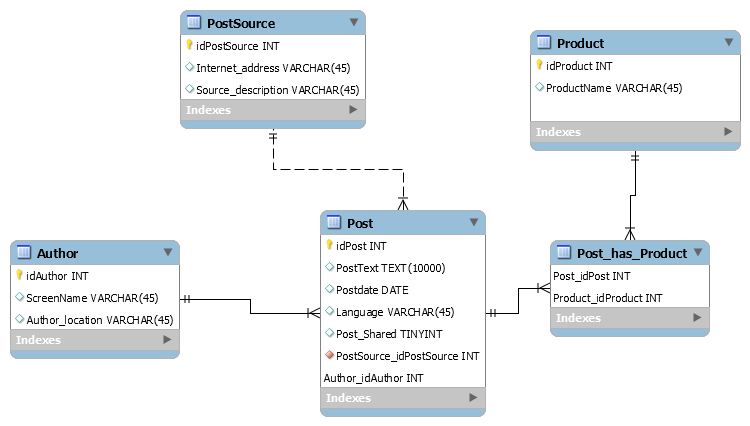
\includegraphics[width=6.5in]{db.png} 
\caption{Schema of a relational database with the posts obtained from multiple sources.}
\label{fig_db} 
\end{figure*}

\section{Methodology}

A potentially faster method of proactively identifying problems with the product is monitoring the user discussion and chat groups.  Multiple websites exist wherein users of Illumina products discuss potential problems with those products and seek solutions (for example, www.seqanswers.com). 

 MySQL was used for demonstrating a schema of a relational database. MySQL is the world's most popular open source database. It is available both in a free of charge version or enterprise edition available to businesses\cite{mysql}. For this project we used MySQL Community Server release 8.0.13. MySQL Workbench was used to generate the schema.


Twitter is an American online news and social networking service on which users post and interact with messages known as "tweets". Tweets were originally restricted to 140 characters, but on November 7, 2017, this limit was doubled for all languages except Chinese, Japanese, and Korean. Registered users can post, like, and retweet tweets, but unregistered users can only read them. Users access Twitter through its website interface, through Short Message Service (SMS) or its mobile-device application software ("app") \cite{wiki-twitter, twitter}. Due to the number of character limits and the information on users provided by the platform, it is ideal for testing the data collection for this project. 

In order to have access to Twitter data programmatically, we created an app that interacts with the Twitter application programming interface (API). There are many APIs on the Twitter platform that software developers can engage with, with the ultimate possibility to create fully automated systems which will interact with Twitter \cite{twitterapi}. For this project we chose the oldest package created for this purpose: Tweepy. It is an easy-to-use Python library for accessing the Twitter API which has extensive documentation and use demonstrations online \cite{tweepy}. 

MongoDB was used to store the information obtained from Twitter. MongoDB is a cross-platform document-oriented database program. Classified as a NoSQL database program, MongoDB uses JSON-like documents with schemata. MongoDB is developed by MongoDB Inc. and licensed under the Server Side Public License (SSPL) \cite{wiki-mongo}.The benefit of MongoDB is that it stores data in flexible, JSON-like documents, meaning fields can vary from document to document and data structure can be changed over time \cite{mongodb}.

Textblob package was used to do the text processing. TextBlob is a Python library for processing textual data. It provides a simple API for diving into common natural language processing (NLP) tasks such as part-of-speech tagging, noun phrase extraction, sentiment analysis, classification, translation, and more \cite{textblob}. The textblob.sentiments module contains two sentiment analysis implementations: PatternAnalyzer (based on the pattern library) and NaiveBayesAnalyzer (an NLTK classifier trained on a movie reviews corpus).




\section{Results}
At the start of the project we created a mock relational database using MySQL. We assumed collection of comments from multiple websites. A post will have an author we likely can identify and track. The same post may mention multiple products made by Illumina. The posts may further be shared by other other users. Technically the same user may be posting on multiple websites, but since aliases are likely to be used, it is unlikely we can track users over multiple websites. The schema is shown in Figure \ref{fig_db}. We can continue expanding the database schema, however, it is unlikely to provide any useful insight into the data contained in the text of the post. We would likely have to perform preprocessing of the text prior to logging the record into the database and add attributes based on the Natural Language processing algorithms. Due to the complexity of connecting to various websites and creating customized scrapers, we did not drive this solution to the full completion in this project. 

Instead of trying to collect information from multiple wesites, we chose instead to concentrate on Twitter to test the data collection and rudimentary NLP processing. We created a Python script utilizing Tweepy package which searched though tweets on Twitter for the following keywords: "Illumina", "MiSeq", "MiniSeq", "NextSeq", "NovaSeq", "iSeq", "HiSeq". By doing this we collected tweets generally discussing Illumina as well as mentioning its DNA sequencing platforms currently available on the market. 

Tweepy returned the following parameters in the Status object: \textit{ 
 \_\_class\_\_,  \_\_delattr\_\_,  \_\_dict\_\_,  \_\_dir\_\_,  \_\_doc\_\_,  \_\_eq\_\_,  \_\_format\_\_, 
 \_\_ge\_\_,  \_\_getattribute\_\_,  \_\_getstate\_\_,  \_\_gt\_\_,  \_\_hash\_\_,  \_\_init\_\_,
 \_\_init\_subclass\_\_,  \_\_le\_\_,  \_\_lt\_\_,  \_\_module\_\_,  \_\_ne\_\_,  \_\_new\_\_,
 \_\_reduce\_\_,  \_\_reduce\_ex\_\_,  \_\_repr\_\_,  \_\_setattr\_\_,  \_\_sizeof\_\_,  \_\_str\_\_,
 \_\_subclasshook\_\_,  \_\_weakref\_\_,  \_api,  \_json,  author,  contributors,  coordinates,
 created\_at,  destroy,  display\_text\_range,  entities,  favorite,  favorite\_count,  favorited,
 full\_text,  geo,  id,  id\_str,  in\_reply\_to\_screen\_name,  in\_reply\_to\_status\_id,
 in\_reply\_to\_status\_id\_str,  in\_reply\_to\_user\_id,  in\_reply\_to\_user\_id\_str,
 is\_quote\_status,  lang,  metadata,  parse,  parse\_list,  place,  retweet,  retweet\_count,
 retweeted,  retweets,  source,  source\_url,  truncated,  user}.

Note that to obtain non-truncated text of the tweets we had to change the default setting of the Tweepy query. If one wants to get full-text on Twitter response, it is necessary to add a keyword tweet\_mode='extended' when calling API. By adding this keyword, obtained full\_text field in the response from the API, instead of text field.

\begin{figure*} 
\centering
\includegraphics[width=5.5in]{sentiment.png} 
\caption{Sentiment alalysis for the selected Illumina products.}
\label{sentiment} 
\end{figure*}

The Status object of tweepy itself is not JSON serializable, but it has a \_json property which contains JSON serializable response data as a dictionary. By using json.dumps(tweet.\_json) command, we extracted all relevant information about every single tweet in JSON format. We saved it on a hard drive for later upload to a database. 

When running the query it was obvious that many of the returned tweets with the same text were repeated multiple time due to retweeting. A Retweet is a re-posting of a Tweet. Twitter's Retweet feature helps you and others quickly share that Tweet with all of your followers \cite{twitter}. Sometimes people type "RT" at the beginning of a Tweet to indicate that they are re-posting someone else's content. This isn't an official Twitter command or feature, but signifies that they are quoting another person's Tweet. Although knowing when specific tweet is being retweeted multiple times is useful for certain applications, we modified the query to eliminate retweets from the results. First we eliminated the tweets starting with "RT" by just checking a tweet's text to see if it starts with 'RT'. Then we eliminated all tweets marked as "retweet".


To analyze the collected data we loaded the information into MongoDB by creating "Illimuna" database with a collection called twitter. To populate the database we used "mongoimport". The "mongoimport" tool imports content from an Extended JSON, CSV, or TSV export created by mongoexport, or potentially, another third-party export tool \cite{mongodb}. Since Twitter allows collecting tweets only for the last 7 days for free accounts, we had to collect the data several time. For subsequent updates of the database we used "upsert" option of the mongoimport. By default, mongoimport uses the \_id field of JSON file to match documents in the collection with documents in the import file. To specify that to match existing documents for the upsert mode, we used --upsertFields with the "id" of the twitter.

For this project we did not do any preprocessing of the text before placing it in the database. Since the dataset is small we can do text analysis on the text queried from the database. For larger dataset a carefully designed preprocessing of the text is needed to avoid long wait time. 

To test the database we created a query in Python which searched through a "full\_text" field for specific keywords, such as product name, and returned only full text of tweets which fit the search criteria. For example when searching for tweets with "novaseq", it will return all tweets which have the word "novaseq" in it. We used "\$regex" operator which provides regular expression capabilities for pattern matching strings in queries. Option "i" makes the query case insensitive. 

One of things which are obvious when we look at the tweets is that they are written in different languages. Therefore, to obtain useful information on all tweets, we utilized a TextBlob "translate" function which automatically detects the source language and translates to the specified language \cite{textblob}. Language translation and detection is powered by the Google Translate API. Although the automatic translation may not be perfect, it can provide us with adequate information for further analysis.

As an example of the data which can be obtained from text analysis we calculated Sentiment of every tweet. Sentiment analysis is basically the process of determining the attitude or the emotion of the writer, i.e., whether it is positive or negative or neutral. Sentiment property of TextBlob returns a namedtuple of the form Sentiment(polarity, subjectivity). Polarity is float which lies in the range of [-1,1] where 1 means positive statement and -1 means a negative statement. 

Figure \ref{sentiment} shows the result of the sentiment analysis returned for NovaSeq and MiSeq products. One can see that in the time frame of the analyzed tweets the majority of the tweets were positive. One can see that there is an outlier for sentiment with the polarity equaling -0.64. We identified the tweet which generated the low polarity score. It stated "\textit{Just shy of 4 TeraBases for our S4 NovaSeq run. That is seriously mad!}" This is obviously not a negative statement as the author is likely expressing amazement at the amount of genetic data his new Illumina instrument is producing. The negative value of the polarity is likely cause by words "shy" and "mad". Further human analysis or machine learning supervised training will be needed to obtain more accurate NLP generated data.  


\section{Conclusions}
We obtained Illumina users' comments from Twitter and organized them in a database. The database can be queried by product allowing for the analysis of consumer sentiment to allow the company to identify potential problems with specific products.




\bibliographystyle{IEEEtran}
\bibliography{Illumina2}

\end{document}